\documentclass[a4paper,DIV=calc,11pt]{scrartcl}
\usepackage[T1]{fontenc}
\usepackage{graphicx}
\usepackage[utf8]{inputenc}
\usepackage[autostyle=true,german=quotes]{csquotes}
\usepackage[english]{babel}
\usepackage[colorlinks=false,pdfborder={0 0 0},bookmarksnumbered]{hyperref}
\usepackage{hyperref}
\usepackage{setspace}
\usepackage[osf]{libertine}
\usepackage{microtype}
\usepackage[ddmmyyyy]{datetime}
\usepackage{amsmath}
\begin{document}


\section*{\# Stay at home --- Are Germany's greenhouse gas emissions increasing or decreasing}

Besides the current Covid-19 issue the population of the whole world is facing the climate change. Almost all human activities cause or lead to greenhouse gas emissions, which drive up the temperature. Extreme weather and melting polar ice are other possible effects. Consequently it is highly relevant to identify economic sectors and human behavior with the potential to decrease emissions.\\

Current research regarding this topic is mostly based on mathematical models and can not be verified by actual data. Due to the restrictions of the Covid-19 crisis the human behavior has transformed, which creates ground truth data and the possibility to conclude how to decease greenhouse gas emissions based on the restrictions of the crisis.\\ On the one hand certain economic sectors can be analysed and potential factors derived, which lead to decreasing emissions. On the other hand the general question \enquote{What can we do?}, which refers to the actions every human can take, can be answered based on actual data.\\

Our group wants to focus on Germany. However, it is possible to answer the question for different countries or areas.\\


\textbf{Aspects our group wants to consider:}\\
In our group were many concerns, if we will find enough information to verify the predictions of our model. So we spend much time to find possible data sources to answer the research question. The task for this milestone is not to find data source, so we decided to group our current sources into general topics

\begin{itemize}
    \item The German \enquote{Umweltbundesamt} is providing actual CO2 data
    \item Real time monitoring of greenhouse gases with satellite pictures
    \item Information from economic sectors can be used as additional predictor --- for example the electricity sector
    \item The consumption of resources (oil, coal,...)
\end{itemize}

\textbf{Project Structure:}\\
We decided to organise our project using a Gantt chart. Where we are including all milestones and additional tasks required to fulfill the each milestone. Fig. \ref{fig:projplan} shows a short overview of the current plan. The last milestone is collapsed to show is clearly.\\

\textbf{Project Organisation:}\\
Beside the Gantt chart we decided to assign specialists to certain tasks (table \ref{tab:special}). The specialists have experience to accomplish the task and therefore they are responsible to keep track of the process and improve the work flow.\\


\begin{table}[ht]
\begin{tabular}{l|l|l}
Task                      & Responsible Person  & Description                             \\ \hline
Data Engineer             & Samra               & Collecting Data, Quality, Preprocessing \\
Machine Learning Engineer & Mohamed, Utku, Noah & Model creation                          \\
Software Engineer         & Mariem              & Front End                               \\
Project Manager           & Zubair              & Planning, Documentation                 \\
Submissions               & Laura, Robert       & Report                                  \\
Video                     & Natalia             &                                        
\end{tabular}
\caption{Project tasks assigned to specialists}
\label{tab:special}
\end{table}
During the project phase we want to have a long planning meeting at the beginning of each milestone to divide the tasks of the milestone into work packages and assign people to them. We do not think it makes sense to assign work packages at the moment, as the project phase has not started and we do not have a topic.\\

\textbf{Risks:}\\
Our group tried to identify possible risks during the project phase. The following list contains the results of a short brainstorming.

\begin{itemize}
    \item Quality of the data
    \item Not enough data
    \item No existing data for performance measurement - No ground truth
    \item We are discussing a complex issue, obtaining clear results can be difficult
    \item No program for video editing
    \item Not enough computing power to train the models
    \item Version control (updates of packages)
    \item Organisational issues (no personal meetings, big group, conflict potentials)
    \item Other lectures (overlapping deadlines)
\end{itemize}

After some discussion we agreed, that the only risk is not to find enough data. The other issues result in additional workload but do not jeopardise the project. However, with the possible data sources mentioned earlier we are confident, that we are well prepared for the project phase.

Additionally our group found a detailed explanation how to structure larger machine learning project and we agreed to follow this guide. (\href{https://www.jeremyjordan.me/ml-projects-guide/}{link})\\





\begin{figure}[ht]
\rotatebox{90}{%
\begin{minipage}{1.5\textwidth}
\centering
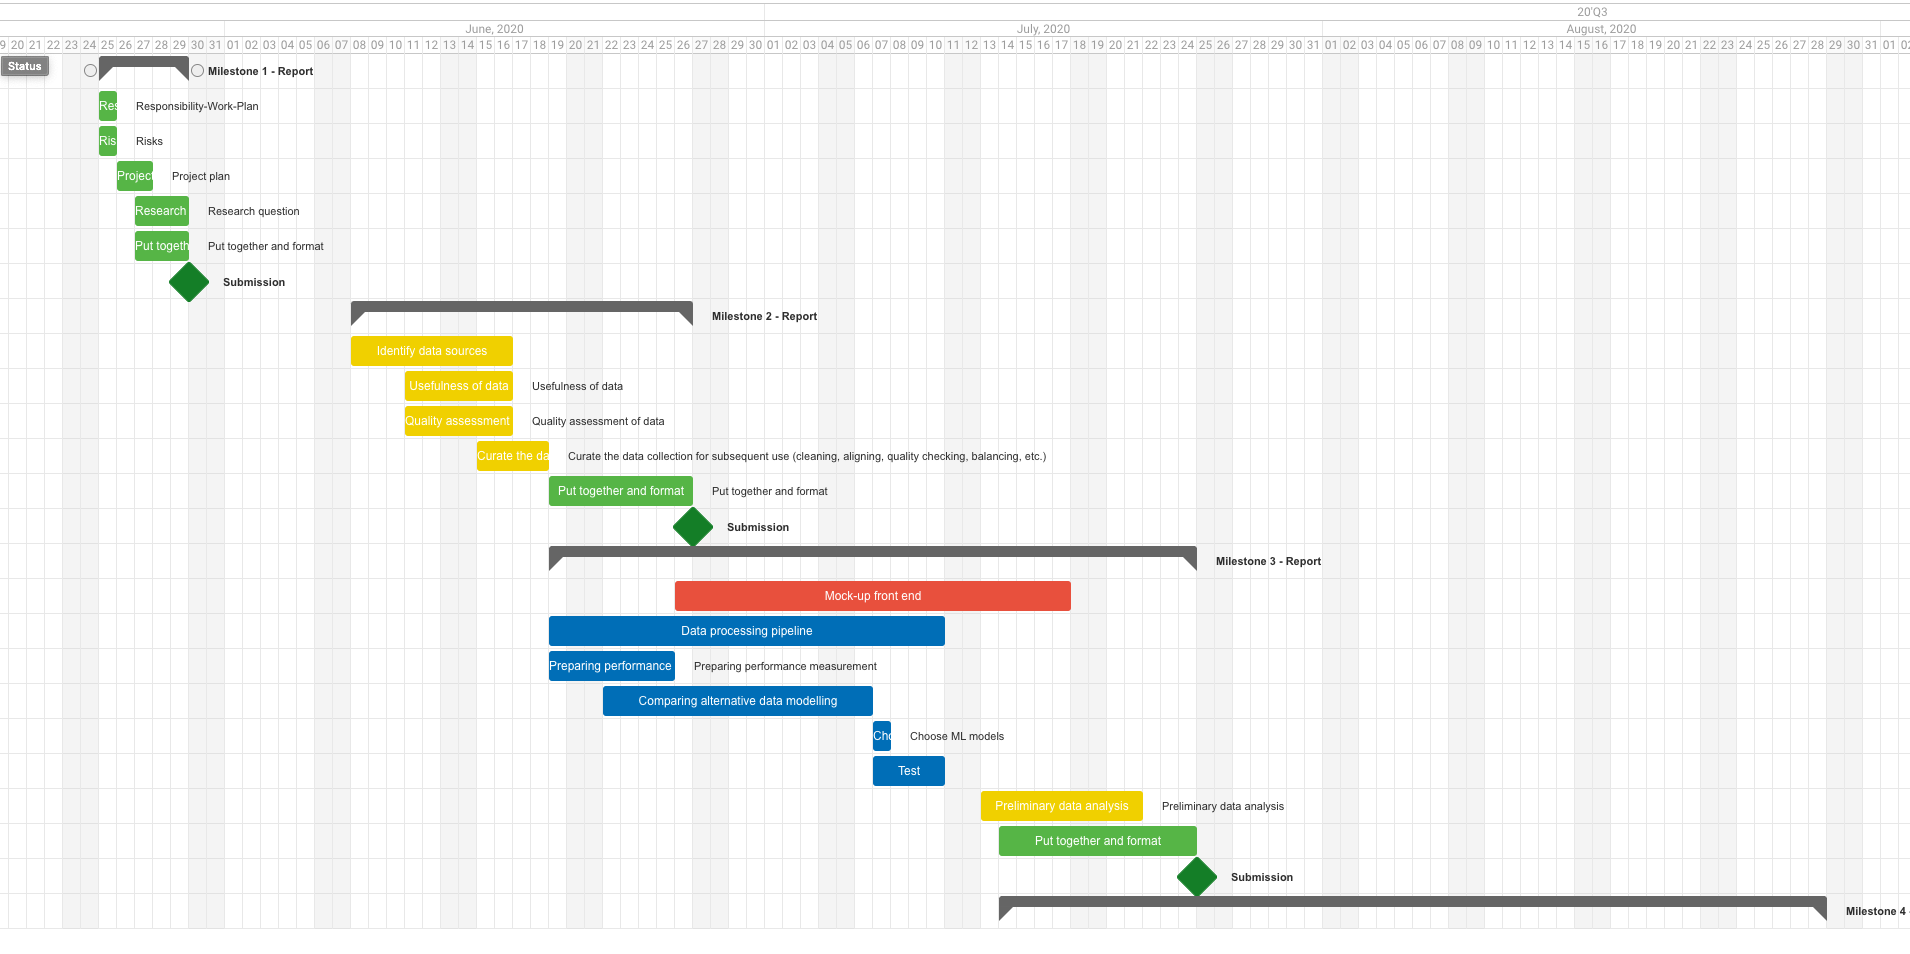
\includegraphics[width=0.99\textwidth]{fig/gantt}
    \caption{Gantt Project Plan (24.05.2020)}%
    \label{fig:projplan}
\end{minipage}
}
\end{figure}

\end{document}
